\section{Attitude Control of Satellite}
\subsection{}
\subsubsection{Finding equilibrium}
We are given the following equations of motion (EoM) for the satellite
\begin{equation}
\label{eq:dynamics}
	\begin{aligned}
		\dot{\mathbf{q}} = \mathbf{T}_q (\mathbf{q} ) \boldsymbol{\omega}, \\
		\mathbf{I}_{CG} \dot{\boldsymbol{\omega}} - \mathbf{S} (\mathbf{I}_{CG} \boldsymbol{\omega} ) \boldsymbol{\omega} & =  \boldsymbol{\tau}.
	\end{aligned}
\end{equation}
To linearize this, we must first find an equilibrium point. We set the derivatives $\dot{\mathbf{q}}$ and $\dot{\boldsymbol{\omega}}$ equal to zero and in addition require $\mathbf{q} = [\eta, \epsilon_1, \epsilon_2, \epsilon_3]^\top  = [\eta, 0, 0, 0]^\top$ and $\boldsymbol{\tau} = \mathbf{0}$ thus obtaining
\begin{align}
\label{eq:ang_vel_trans_1}
\mathbf{T_q}(\mathbf{q})\boldsymbol{\omega}_0 = \mathbf{0}, \\
\label{eq:ang_vel_trans_2}
\mathbf{S}(\mathbf{I}_{CG} \boldsymbol{\omega}_0)\boldsymbol{\omega}_0 = \mathbf{0}.
\end{align}
Using (2.69) from \cite{Fossen2011} we can rewrite \eqref{eq:ang_vel_trans_1} and obtain
\begin{equation}\begin{aligned}
\mathbf{T_q}(\mathbf{q})\boldsymbol{\omega}_0
&= \frac{1}{2}
\begin{bmatrix}
- \boldsymbol{\epsilon}_0^\top \\
\eta \mathbf{I}_3 + \mathbf{S}(\boldsymbol{\epsilon}_0)
\end{bmatrix}
\boldsymbol{\omega}_0 \\
&= \frac{1}{2}
\begin{bmatrix}
\mathbf{0}^\top \\
\mathbf{I}_3
\end{bmatrix}
\boldsymbol{\omega}_0 \\
&= \mathbf{0}.
\end{aligned}\end{equation}
Hence $\boldsymbol{\omega}_0 = \mathbf{0}^\top$ and we have the equilibrium point $\mathbf{x}_0 = [\boldsymbol{\epsilon}_0^\top, \boldsymbol{\omega}_0^\top]^\top = \mathbf{0}^\top$. This clearly also satisfies \eqref{eq:ang_vel_trans_2}.
\subsubsection{Linearizing around equilibrium}
We wish to linearize this non-linear system around $\mathbf{x}_0$. For that, we need expressions for $\dot{\boldsymbol{\epsilon}}$ and $\dot{\boldsymbol{\omega}}$. We find
\begin{align}
\dot{\boldsymbol{\epsilon}}
&= \frac{1}{2}(\eta \mathbf{I}_3 + \mathbf{S}(\boldsymbol{\epsilon}))\boldsymbol{\omega}
= \frac{1}{2}\eta \boldsymbol{\omega} + \frac{1}{2}\mathbf{S}(\boldsymbol{\omega})\boldsymbol{\omega}
= \frac{1}{2}\eta \boldsymbol{\omega}
= \frac{1}{2}\sqrt{1 - \boldsymbol{\epsilon}^\top\boldsymbol{\epsilon}}\boldsymbol{\omega}, \quad \text{and} \\
\dot{\boldsymbol{\omega}}
&= \mathbf{I}_{CG}^{-1}(\mathbf{S}(\mathbf{I}_{CG}\boldsymbol{\omega})\boldsymbol{\omega} + \boldsymbol{\tau})
=\frac{1}{mr^2}(\mathbf{S}(\mathbf{I}_{CG}\boldsymbol{\omega})\boldsymbol{\omega} + \boldsymbol{\tau})
= \boldsymbol{S}(\boldsymbol{\omega})\boldsymbol{\omega} + \frac{1}{mr^2}\boldsymbol{\tau}
= \frac{1}{mr^2}\boldsymbol{\tau}.
\end{align}
So,
\begin{equation}\begin{aligned}
\dot{\mathbf{x}} =
\begin{bmatrix}
\dot{\boldsymbol{\epsilon}}\\
\dot{\boldsymbol{\omega}}\\
\end{bmatrix}
=\begin{bmatrix}
\frac{1}{2}\sqrt{1-\boldsymbol{\epsilon}^\top\boldsymbol{\epsilon}}\boldsymbol{\omega}\\
\frac{1}{mr^2}\boldsymbol{\tau}\\
\end{bmatrix}
= \mathbf{f}(\mathbf{x}, \boldsymbol{\tau}).
\end{aligned}\end{equation}
The linearized system has the form
\begin{equation}\begin{aligned}
\dot{\hat{\mathbf{x}}} = \mathbf{A}\hat{\mathbf{x}} + \mathbf{B}\hat{\boldsymbol{\tau}}
\end{aligned}\end{equation}
where $\mathbf{A} = $ and $\mathbf{B}$ are the Jacobians $\frac{\partial \mathbf{f}}{\partial \mathbf{x}}$, and $\frac{\partial \mathbf{f}}{\partial \boldsymbol{\tau}}$ respectively, evaluated at the equilibrium $\mathbf{x}=\mathbf{x_0}$. That is,
\begin{align}
\label{eq:A_matrix}
\mathbf{A}
&= \begin{bmatrix}
-\frac{1}{2}\sqrt{1-\boldsymbol{\epsilon}_0^\top\boldsymbol{\epsilon}_0}\boldsymbol{\epsilon}_0\boldsymbol{\omega}_0^\top & \frac{1}{2}\sqrt{1-\boldsymbol{\epsilon}_0^\top\boldsymbol{\epsilon}_0}\mathbf{I}_3\\
\mathbf{0}_3 & \mathbf{0}_3 \\
\end{bmatrix}
= \begin{bmatrix}
\mathbf{0}_3 & \frac{1}{2}\mathbf{I}_3 \\
\mathbf{0}_3 & \mathbf{0}_3 \\
\end{bmatrix}, \quad \text{and} \\
\mathbf{B}
\label{eq:B_matrix}
&= \begin{bmatrix}
\mathbf{0}_3\\
\frac{1}{mr^2}\mathbf{I}_3\\
\end{bmatrix}
\end{align}
where $\mathbf{0}_3$ denotes a 3-by-3 zero-valued matrix. \eqref{eq:A_matrix} follows from the following results
\begin{align}
\frac{\partial}{\partial \epsilon_i}\frac{1}{2}\sqrt{1-\epsilon_1^2 - \epsilon_2^2 - \epsilon_3^2}\omega_k
&= -\frac{1}{2}\sqrt{1-\epsilon_1^2 - \epsilon_2^2 - \epsilon_3^2}^{-1}\epsilon_i \omega_k, \\
\frac{\partial}{\partial \omega_i}\frac{1}{2}\sqrt{1-\boldsymbol{\epsilon}^\top\boldsymbol{\epsilon}}\omega_i
&=\frac{1}{2}\sqrt{1-\boldsymbol{\epsilon}^\top\boldsymbol{\epsilon}}.
\end{align}


\subsection{}
We now introduce the control law
\begin{equation}
  \label{eq:control_law}
  \mathbf{\tau} = -\mathbf{K}_d \boldsymbol{\omega} - k_p \boldsymbol{\epsilon},
\end{equation}
where $\mathbf{K}_d = k_d \mathbf{I}_3 = 40 \mathbf{I}_3$ and $k_p = 2$. Since this input is only dependent on our state vector $x$, we can find an expression for the closed loop system with a single system matrix. This system becomes
\begin{equation}\begin{aligned}
\dot{\hat{ \mathbf{x}}}
&= \mathbf{A}\hat{\mathbf{x}} + \mathbf{B}\hat{\boldsymbol{\tau}} \\
&= \mathbf{A}\hat{\mathbf{x}} + \mathbf{B}(-\mathbf{K}_d \boldsymbol{\omega} - k_p \boldsymbol{\epsilon}) \\
&= \mathbf{A}\hat{\mathbf{x}} + \mathbf{B}(
-\begin{bmatrix}
\mathbf{0}_3 & \mathbf{K}_d \\
\end{bmatrix} \hat{\mathbf{x}}
-\begin{bmatrix}
k_p \mathbf{I}_3 & \mathbf{0}_3 \\
\end{bmatrix}\hat{\mathbf{x}}
) \\
&= (\mathbf{A}\hat{\mathbf{x}} - \mathbf{B}
\begin{bmatrix}
k_p \mathbf{I}_3 & \mathbf{K}_d \\
\end{bmatrix}
) \hat{\mathbf{x}} \\
&= \left(
\begin{bmatrix}
\mathbf{0}_3 & \frac{1}{2}\mathbf{I}_3 \\
\mathbf{0}_3 & \mathbf{0}_3 \\
\end{bmatrix}
-
\begin{bmatrix}
\mathbf{0}_3\\
\frac{1}{mr^2}\mathbf{I}_3\\
\end{bmatrix}
\begin{bmatrix}
k_p\mathbf{I}_3 & \mathbf{K}_d \\
\end{bmatrix}
\right) \hat{\mathbf{x}} \\
&=
\begin{bmatrix}
\mathbf{0}_3 & \frac{1}{2}\mathbf{I}_3 \\
-\frac{k_p}{mr^2}\mathbf{I}_3& -\frac{1}{mr^2}\mathbf{K}_d \\
\end{bmatrix}
\hat{\mathbf{x}}.
\end{aligned}\end{equation}
The matlab command below is used to find the eigenvalues of this matrix, which will coincide with the poles of the closed loop transfer function.
\lstset{language=Matlab, basicstyle=\small}
\begin{lstlisting}[frame=single]
eigs([zeros(3,3), 1/2*eye(3); -k_p/(m*r^2)*eye(3), -k_d/(m*r^2)*eye(3)])
\end{lstlisting}
These eigenvalues are found to be $\lambda_{1,2} = -0.0278 \pm 0.0248j$, i.e. complex conjugated in the left half plane. This means that the system is stable. \textbf{TODO: Do we want complex conjugated or real?}

\subsection{}
With the control law from \eqref{eq:control_law} the system behaves as shown in figure \ref{fig:zero_control_law}. This control law drives the euler angles to zero. To drive them to an arbitrarily chosen reference $\boldsymbol{\epsilon}$, we would instead have to define the control law using the reference error $\tilde{\boldsymbol{\epsilon}}$, as is done in equation (3).
\begin{figure}[ht]
	\centering
	\begin{subfigure}[b]{0.45\textwidth}
		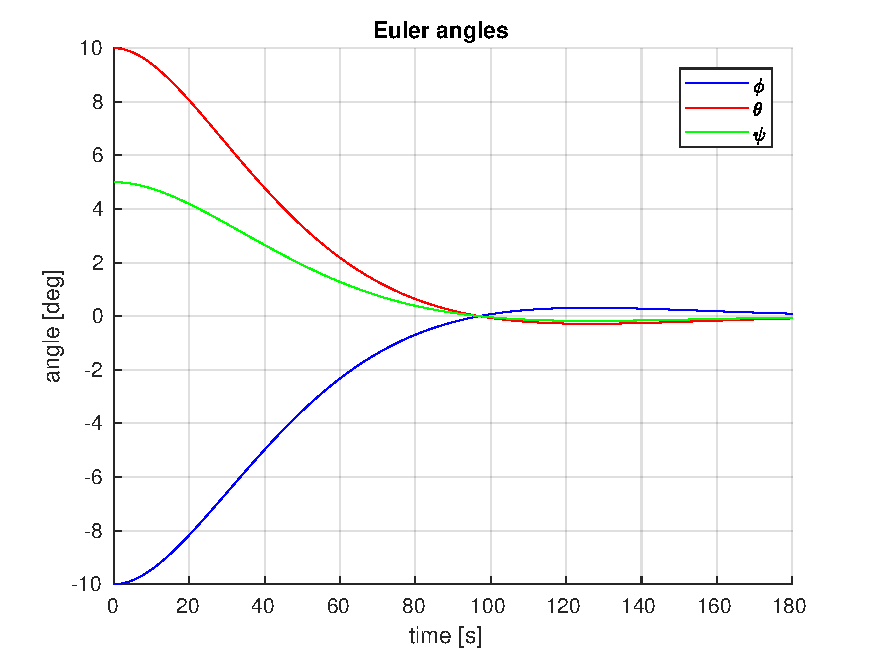
\includegraphics[width=\textwidth]{1_3_euler_angles}
		\caption{Euler angles.}
		\label{fig:2a}
	\end{subfigure}
	~ %add desired spacing between images, e. g. ~, \quad, \qquad, \hfill etc.
	%(or a blank line to force the subfigure onto a new line)
	\begin{subfigure}[b]{0.45\textwidth}
		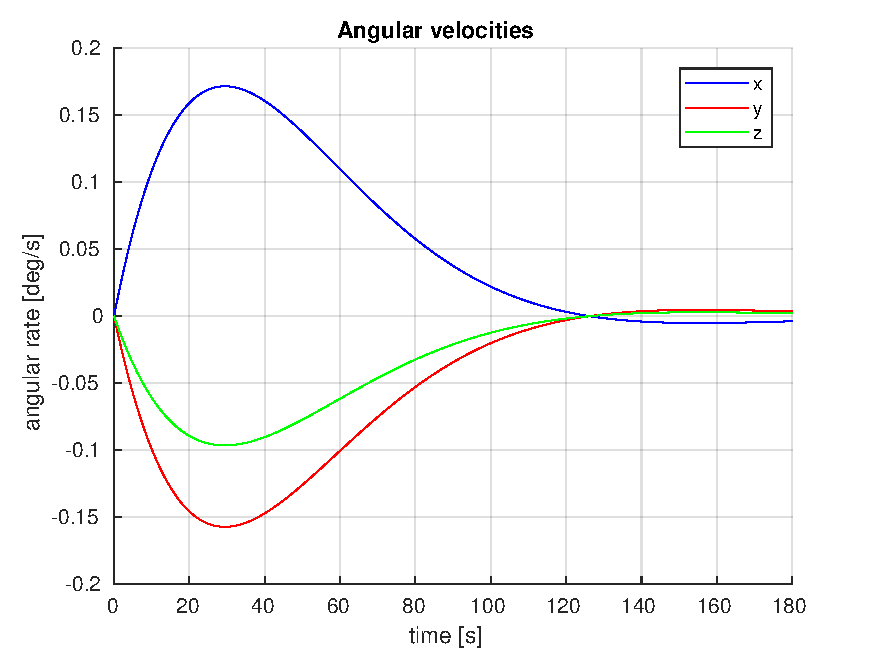
\includegraphics[width=\textwidth]{1_3_angular_velocities}
		\caption{Angular velocities.}
		\label{fig:2b}
	\end{subfigure}
	\begin{subfigure}[b]{0.45\textwidth}
		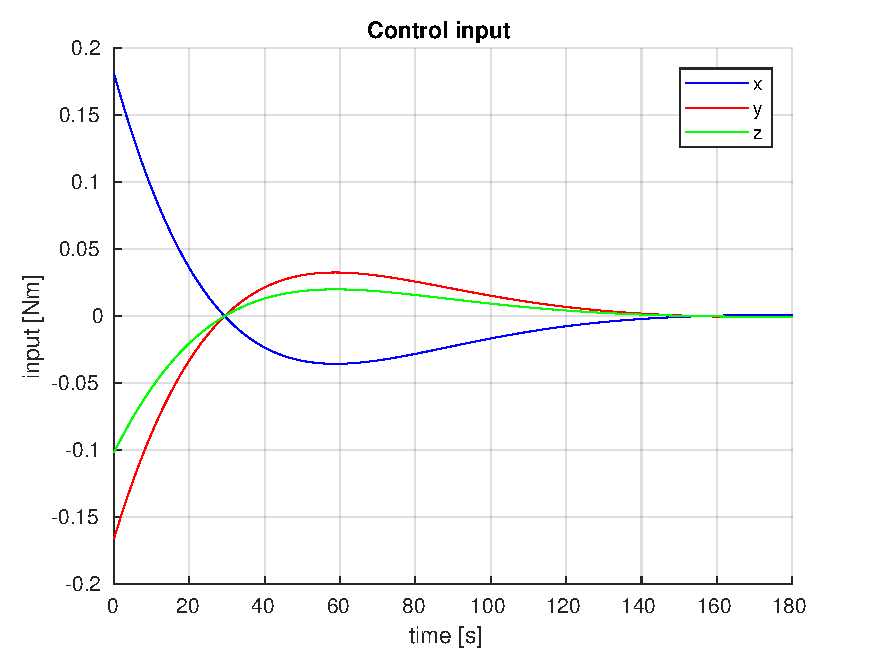
\includegraphics[width=\textwidth]{1_3_control_input}
		\caption{Control input.}
		\label{fig:2c}
	\end{subfigure}
	\caption{Simulation results with control law \eqref{eq:control_law}}\label{fig:zero_control_law}
\end{figure}

\subsection{}
To make a control law based on deviation from a reference, we define the quaternion error
 \begin{equation}
	 \tilde{\mathbf{q}} := \left[
	 \begin{array}{c}
		 \tilde{\eta} \\
		 \tilde{\epsilon}
	 \end{array}
	 \right] = \bar{\mathbf{q}}_d \otimes \mathbf{q},
 \end{equation}
where $\mathbf{q}_d$ is the reference (and the bar denotes the quaternion conjugate). Using the definition of the quaternion product from the assignment text, we obtain
\begin{equation}\begin{aligned}
\tilde{\mathbf{q}} =
\begin{bmatrix}
\eta_d \eta + \boldsymbol{\epsilon}^\top_d \boldsymbol{\epsilon}\\
\eta_d \boldsymbol{\epsilon} - \eta \boldsymbol{\epsilon}_d - \mathbf{S}(\boldsymbol{\epsilon}_d)\boldsymbol{\epsilon}\\
\end{bmatrix}
=
\begin{bmatrix}
\eta_d \eta + \epsilon_{d1} \epsilon_1 + \epsilon_{d2}\epsilon_2 + \epsilon_{d3}\epsilon_3\\
\eta_d \epsilon_1 - \eta \epsilon_{d1} - \epsilon_{d2} \epsilon_3 + \epsilon_{d3}\epsilon_2 \\
\eta_d \epsilon_2 - \eta \epsilon_{d2} - \epsilon_{d3} \epsilon_1 + \epsilon_{d1}\epsilon_3 \\
\eta_d \epsilon_3 - \eta \epsilon_{d3} - \epsilon_{d1} \epsilon_2 + \epsilon_{d2}\epsilon_1 \\
\end{bmatrix}
\end{aligned}\end{equation}
where we have used
\begin{equation}\begin{aligned}
\mathbf{S}(\epsilon_d)\epsilon =
\begin{bmatrix}
0 & -\epsilon_{d3} & \epsilon_{d2}\\
\epsilon_{d3} & 0 & -\epsilon_{d1} \\
-\epsilon_{d2} & \epsilon_{d1} & 0 \\
\end{bmatrix}
\begin{bmatrix}
\epsilon_1\\
\epsilon_2\\
\epsilon_3\\
\end{bmatrix}
=
\begin{bmatrix}
\epsilon_{d2} \epsilon_3 - \epsilon_{d3}\epsilon_2\\
\epsilon_{d3} \epsilon_1 - \epsilon_{d1}\epsilon_3\\
\epsilon_{d1} \epsilon_2 - \epsilon_{d2}\epsilon_1\\
\end{bmatrix}.
\end{aligned}\end{equation}
After convergence, i.e. when $\mathbf{q} = \mathbf{q}_d$, this error becomes
\begin{equation}\begin{aligned}
\tilde{\mathbf{q}} =
\begin{bmatrix}
\eta_d^2 + \boldsymbol{\epsilon}^\top_d \boldsymbol{\epsilon}_d\\
\eta_d \boldsymbol{\epsilon}_d - \eta_d \boldsymbol{\epsilon}_d - \mathbf{S}(\boldsymbol{\epsilon}_d)\boldsymbol{\epsilon}_d\\
\end{bmatrix}
=
\begin{bmatrix}
1\\
\mathbf{0}\\
\end{bmatrix}
\end{aligned}\end{equation}
since $\eta^2 = 1 - \boldsymbol{\epsilon}^\top \boldsymbol{\epsilon}$ and $\boldsymbol{\mathbf{S}}(\boldsymbol{\epsilon})\boldsymbol{\epsilon} = \mathbf{0}$.

\subsection{}
We now try to simulate with the control law based on a reference $\mathbf{q}_d$, i.e. with the control law
\begin{equation}\begin{aligned}
\label{eq:control_law_error}
\boldsymbol{\tau} = - \mathbf{K}_d -k_p \tilde{\boldsymbol{\epsilon}}.
\end{aligned}\end{equation}
\begin{figure}[H]
	\centering
	\begin{subfigure}[b]{0.45\textwidth}
		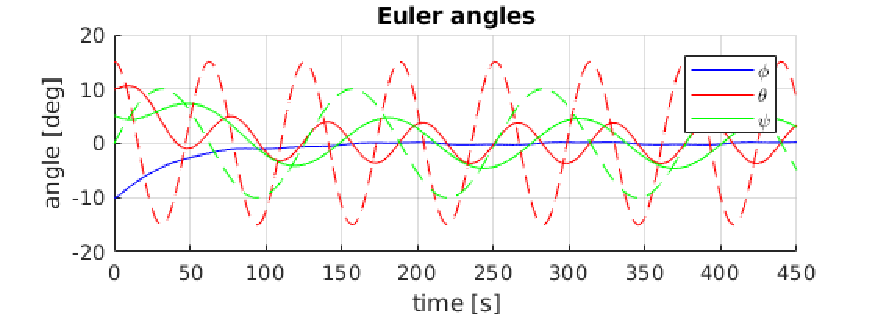
\includegraphics[width=\textwidth]{../matlab/1_5_euler_angles}
		\caption{Euler angles. Reference: dashes, state: line.}
		\label{fig:5a}
	\end{subfigure}
	~ %add desired spacing between images, e. g. ~, \quad, \qquad, \hfill etc.
	%(or a blank line to force the subfigure onto a new line)
	\begin{subfigure}[b]{0.45\textwidth}
		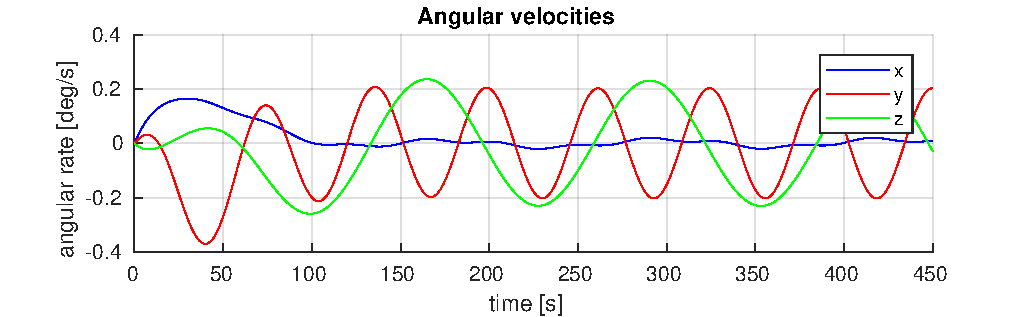
\includegraphics[width=\textwidth]{../matlab/1_5_angular_velocities}
		\caption{Angular velocities.}
		\label{fig:5b}
	\end{subfigure}
	\begin{subfigure}[b]{0.45\textwidth}
		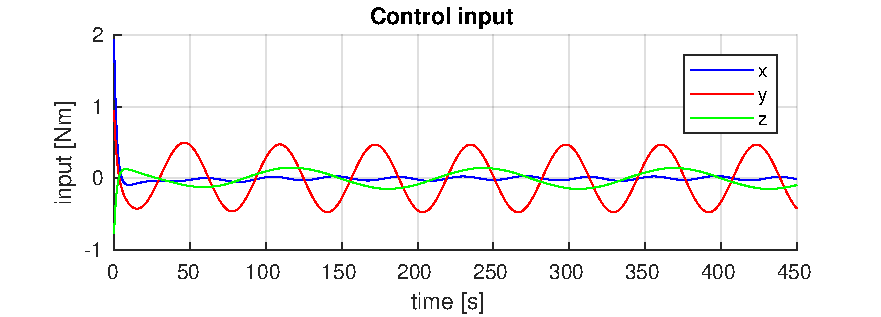
\includegraphics[width=\textwidth]{../matlab/1_5_control_input}
		\caption{Control input.}
		\label{fig:5c}
	\end{subfigure}
	\begin{subfigure}[b]{0.45\textwidth}
		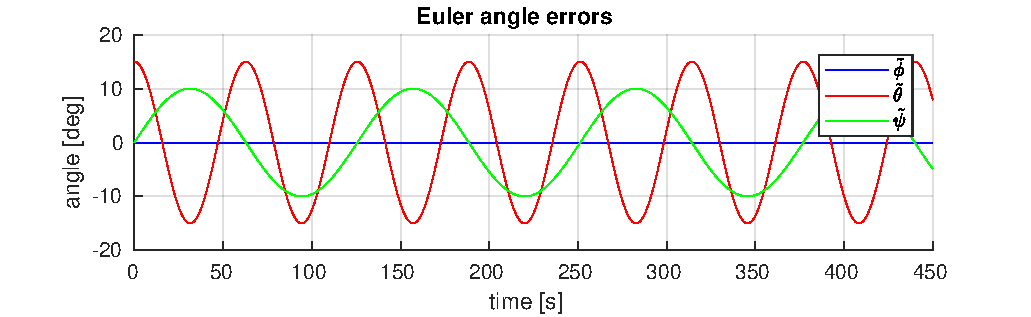
\includegraphics[width=\textwidth]{../matlab/1_5_euler_angle_errors}
		\caption{Error in euler angles.}
		\label{fig:5d}
	\end{subfigure}
	\caption{Simulation results with control law \eqref{eq:control_law_error}}\label{fig:error_control_law}
\end{figure}
Figure \ref{fig:error_control_law} shows the system simulated with reference angles $\phi(t) = 0$, $\theta(t) = 15\cos(0.1t)$, $\psi(t) = 10\sin(0.05t)$. As we can see, the satellite is not able to respond to the fast frequencies, so we get a large phase shift and a big decrease in amplitude. We recall that when a sinusoidal signal is differentiated, or passed through a first order system for that matter, the output is scaled proportional to the period, which in this case is quite small, leading to a decreased amplitude.

\subsection{}
We now introduce an angular velocity reference $\boldsymbol{\omega}_d$ to our control law. We define the error of this as $\tilde{\boldsymbol{ \omega}} =\boldsymbol{\omega} - \boldsymbol{\omega}_d$ and the new control law as
\begin{equation}
\label{eq:control_law_ang_error}
	\boldsymbol{\tau} = -\mathbf{K}_d \tilde{\boldsymbol{\omega}} - k_p \tilde{\boldsymbol{\epsilon}}.
\end{equation}
From equation (2.31) in \cite{Fossen2011} we have the following expression for the reference,
\begin{equation}
	\boldsymbol{\omega}_d = \mathbf{T}^{-1}_{\Theta_d}(\Theta_d)\dot{\Theta}_d,
\end{equation}
where $\mathbf{T}^{-1}_{\boldsymbol{\Theta}_d}$, given by equation (2.33), is
\begin{equation}\begin{aligned}
\mathbf{T}^{-1}_{\boldsymbol{\Theta}_d} =
\begin{bmatrix}
1 & 0 & -\sin(\theta_d) \\
0 & \cos(\phi_d) & \cos(\theta_d)\sin(\phi_d) \\
0 & \sin(\phi_d) & \cos(\theta_d)\cos(\phi_d) \\
\end{bmatrix}.
\end{aligned}\end{equation}
We analytically differentiate our reference euler angle signals to obtain
\begin{equation}\begin{aligned}
\dot{\boldsymbol{\Theta}_d} =
\begin{bmatrix}
\dot \phi_d\\
\dot \theta_d\\
\dot \psi_d \\
\end{bmatrix} =
\begin{bmatrix}
0\\
-1.5 \sin(0.1t)\\
0.5 \cos(0.05t)\\
\end{bmatrix}.
\end{aligned}\end{equation}
Simulating the system this reference and control law as well as $\mathbf{K}_d = k_d \mathbf{I}_3 = 400 \mathbf{I}_3$ and $k_p = 20$ as before, yields the results shown in figure \ref{fig:ang_error_control_law}.
\begin{figure}[H]
	\centering
	\begin{subfigure}[b]{0.45\textwidth}
		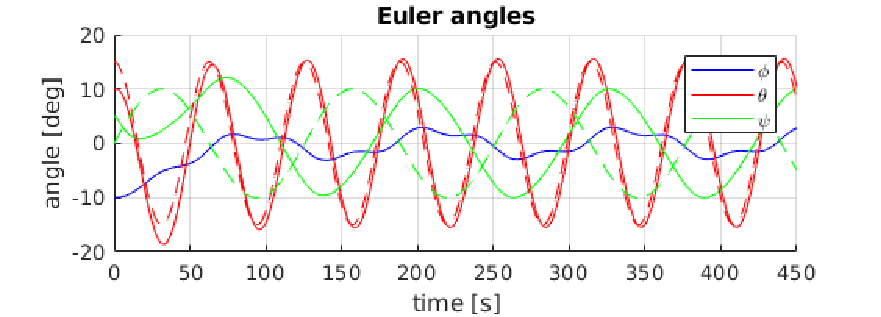
\includegraphics[width=\textwidth]{../matlab/1_6_euler_angles}
		\caption{Euler angles. Reference: dashes, state: line.}
		\label{fig:5a}
	\end{subfigure}
	~ %add desired spacing between images, e. g. ~, \quad, \qquad, \hfill etc.
	%(or a blank line to force the subfigure onto a new line)
	\begin{subfigure}[b]{0.45\textwidth}
		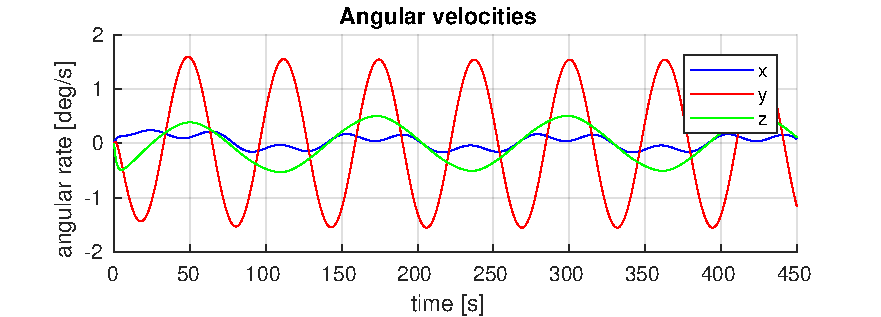
\includegraphics[width=\textwidth]{../matlab/1_6_angular_velocities}
		\caption{Angular velocities.}
		\label{fig:5b}
	\end{subfigure}
	\begin{subfigure}[b]{0.45\textwidth}
		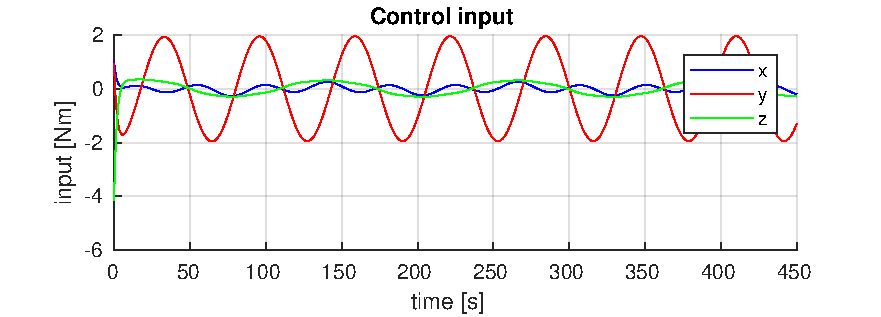
\includegraphics[width=\textwidth]{../matlab/1_6_control_input}
		\caption{Control input.}
		\label{fig:5c}
	\end{subfigure}
	\begin{subfigure}[b]{0.45\textwidth}
		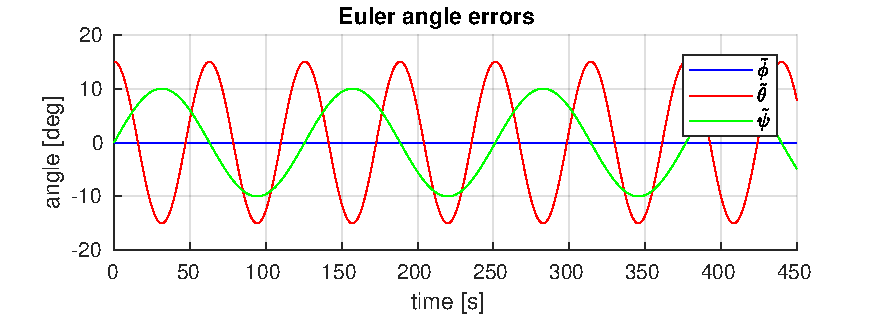
\includegraphics[width=\textwidth]{../matlab/1_6_euler_angle_errors}
		\caption{Error in euler angles.}
		\label{fig:5d}
	\end{subfigure}
	\caption{Simulation results with control law \eqref{eq:control_law_ang_error}}\label{fig:ang_error_control_law}
\end{figure}
This time, the satellite is able to follow the reference very closely in $\theta$. In $\psi$ however, it manages to correctly follow the amplitude, but still has a significant phase shift. The improved performance is very much expected. The previous control law would constantly try to drive the angular velocity to zero. This is clearly unattainable if the satellite is supposed to follow a sineusoidal signal, as its angular velocity would also have to vary with a sine. Since we are able to find the analytical expression for this expected velocity, we can expect great improvements over the earlier control law, and as we have seen, we were able to obtain correct amplitude control.

\subsection{}
We now assume setpoint regulation, i.e. $\boldsymbol{\omega}_d = \mathbf{0}$ and $\boldsymbol{\epsilon}_d$ and $\eta_d$ are constant. The Lyapunov function for this situation can be written as
 \begin{equation}
	 V = \frac{1}{2} \tilde{\boldsymbol{\omega}}^{\top} \mathbf{I}_{CG}\tilde{\boldsymbol{\omega}} + 2 k_p (1-\tilde{\eta})
 \end{equation}
and the derivative as
\begin{equation}
	\dot{V} = -k_d \boldsymbol{\omega}^{\top} \boldsymbol{\omega}.
\end{equation}
We know this to be a Lyapunov function because it is positive. Clearly $\tilde{\boldsymbol{\omega}}^\top\mathbf{I}_{CG}\boldsymbol{\tilde \omega}$ is positive, since $\mathbf{I}_{CG} = mr^2\mathbf{I}$ is positive definite. Furthermore, we have for any quaternion that
\begin{equation}\begin{aligned}
||\mathbf{q}|| = 1 = \sqrt{\eta^2 + \epsilon_1^2 + \epsilon_2^2 + \epsilon_3^2}
= \sqrt{\eta^2 + \boldsymbol{\epsilon}^\top \boldsymbol{\epsilon}}
\end{aligned}\end{equation}
and so
\begin{equation}\begin{aligned}
||\mathbf{q}||^2 = \eta^2 \boldsymbol{\epsilon}^\top\boldsymbol{\epsilon} = 1
\implies \boldsymbol{\epsilon}^\top \boldsymbol{\epsilon} = 1 - \eta^2 \leq 1
\end{aligned}\end{equation}
which further implies
\begin{equation}\begin{aligned}
\eta^2 = 1 - \boldsymbol{\epsilon}^\top \boldsymbol{\epsilon}
\implies \eta = \sqrt{1 - \boldsymbol{\epsilon}^\top \boldsymbol{\epsilon}} \leq 1.
\end{aligned}\end{equation}
Now since $\tilde{\mathbf{q}}$ is a unit quaternion (it is the product of two unit quaternions, which we know map (doubly) to SO(3) and it is closed under multiplication \cite{Sola}), we have $\tilde \eta \leq 1$ and hence $2k_p(1-\tilde \eta)$ is also positive and so $V \geq 0$ always.
